% ============================================================
%  HCMUT-DEE Thesis Kit v2.0.4 — Main Document
%  Copyright (c) 2026 Nguyễn Trọng Thắng & TS. Nguyễn Phúc Khải
%  License: MIT
% ============================================================
%
% HUONG DAN NHANH:
%   1. Chinh sua THONG TIN SINH VIEN o phan ben duoi
%   2. Viet noi dung cac chuong trong folder chapters/
%   3. Bien dich: pdflatex -> bibtex -> pdflatex x2
%
% TUY CHON DOCUMENTCLASS:
%   [vietnamese] (mac dinh) | [english] | [french]
%   [oneside]   (mac dinh, xem tren man hinh)
%   [twoside]   (in 2 mat, dong gay sach)
% ============================================================

% === CHON CHE DO ===
% De in 2 mat: doi thanh [vietnamese, twoside, openright]
\documentclass[vietnamese, oneside]{hcmut-dee}

% ═══════════════════════════════════════════════════════════════
%  THONG TIN SINH VIEN — CHI CHINH SUA PHAN NAY
% ═══════════════════════════════════════════════════════════════

% --- BAT BUOC ---
\ThesisTitle{Tên đề tài bằng tiếng Việt của bạn}
\ThesisTitleEN{Your Thesis Title in English}
\StudentName{Nguyễn Văn A}
\StudentID{xxxxxxx}
\StudentClass{DDxxKTDxx}
\Major{Kỹ thuật Điện}
\Supervisor{TS. Nguyễn Văn B}

% --- TUY CHON (bo comment neu can) ---
% \Faculty{Khoa Điện - Điện Tử}          % Mac dinh da co
% \Department{Bộ môn Hệ thống điện}      % Neu can ghi Bo mon
% \ReportType{ĐỒ ÁN TỐT NGHIỆP}        % Mac dinh da co
\ThesisMonth{06}
\ThesisYear{2026}
\AssignDate{26}{01}{2026}                 % Ngay giao nhiem vu
\DueDate{15}{05}{2026}                    % Ngay hoan thanh
%\Reviewer{TS. Trần Văn C}              % Phan bien (neu biet)
% \SupervisorPercent{100\%}               % Mac dinh 100%
% --- THANH PHAN HOI DONG CHAM (bo comment de dien ho ten neu muon) ---
% \CouncilMemberOne{PGS. TS. Lê Văn D}        % Chu tich Hoi dong
% \CouncilMemberTwo{TS. Nguyễn Văn E}         % Uy vien / Thu ky
% \CouncilMemberThree{TS. Phạm Văn F}        % Uy vien
% \CouncilMemberFour{ThS. Do Van G}           % Uy vien
% \CouncilMemberFive{ThS. Tran Van H}         % Uy vien

% --- NHIEM VU KHOA LUAN (noi dung muc 2 trong trang Nhiem vu) ---
\AssignmentTasks{%
  \begin{itemize}[nosep, leftmargin=1.5em, label={-}, topsep=3pt]
    \item Nghiên cứu tổng quan về \ldots
    \item Xây dựng mô hình toán học cho \ldots
    \item Mô phỏng và đánh giá kết quả trên \ldots
    \item Phân tích và thảo luận kết quả đạt được.
  \end{itemize}
}

% ═══════════════════════════════════════════════════════════════
%  CẤU HÌNH PDF METADATA & HYPERLINK (BẢN QUYỀN & THAM CHIẾU)
% ═══════════════════════════════════════════════════════════════
% Cấu hình các thuộc tính Metadata của file PDF xuất ra (nhấp chuột phải vào 
% file PDF -> Properties để xem) và định dạng màu sắc cho các hyperlink.
\hypersetup{
  unicode=true,
  pdftitle={\getThesisTitle},
  pdfauthor={\getStudentName},
  pdfsubject={\getReportType\ - Ngành \getMajor},
  pdfkeywords={HCMUT, DEE, \getMajor, Đồ án tốt nghiệp, Thesis Kit},
  pdfcreator={HCMUT-DEE Thesis Kit v2.0.4},
  pdfproducer={Copyright (c) 2026 Nguyễn Trọng Thắng và TS. Nguyễn Phúc Khải. MIT License.},
  % Cấu hình hyperlink màu sắc theo quy chuẩn
  colorlinks=true,
  linkcolor=black,             % Màu liên kết nội bộ (Mục lục, hình vẽ, bảng biểu)
  citecolor=red,               % Màu liên kết tài liệu tham khảo (Citation)
  urlcolor=BKBlue              % Màu liên kết link web ngoài (GitHub, các URL khác)
}

% ═══════════════════════════════════════════════════════════════
%  BAT DAU TAI LIEU
% ═══════════════════════════════════════════════════════════════
\begin{document}

% Fix loi trung so trang giua bia va noi dung
\pagenumbering{alph}

% ─── TRANG BIA & GIAY TO CHINH THUC ─────────────────────────
\makecover

\cleardoublepage
\makeassignment

\cleardoublepage
\makeevaluation

% ─── GIAN DONG 1.5 CHO PHAN NOI DUNG ────────────────────────
\onehalfspacing

% So trang La Ma cho phan dau
\pagenumbering{roman}

% ─── LOI CAM ON ──────────────────────────────────────────────
\cleardoublepage
% ============================================================
%  HCMUT-DEE Thesis Kit v2.0.3 — Lời cảm ơn
%  Copyright (c) 2026 Nguyen Trong Thang & TS. Nguyen Phuc Khai
%  License: MIT
% ============================================================

\chapter*{LỜI CẢM ƠN}
\addcontentsline{toc}{chapter}{Lời cảm ơn}

% ═══════════════════════════════════════════════════════════════
%  HUONG DAN: Viet loi cam on cua ban o day.
%  Thuong bao gom:
%    - Cam on Khoa, Truong
%    - Cam on GVHD (ten cu the)
%    - Cam on gia dinh, ban be
%    - Nhan xet ve han che cua do an
%    - Ky ten
%
%  Luu y: Giu van phong trang trong, chan thanh.
%  Do dai khuyen nghi: 1-2 trang.
% ═══════════════════════════════════════════════════════════════

Trước hết, em \textit{Nguyễn Trọng Thắng} - xin bày tỏ lòng biết ơn sâu sắc đến Ban Giám hiệu Trường Đại học Bách Khoa - ĐHQG-HCM, Ban Chủ nhiệm Khoa Điện - Điện tử, cùng toàn thể các thầy cô giáo đã tận tình truyền đạt kiến thức, nâng đỡ và dạy dỗ em trong suốt những năm tháng học tập dưới mái trường Bách Khoa thân yêu.

Đặc biệt, em xin gửi lời tri ân chân thành nhất tới các Thầy Cô giáo tại Bộ môn Hệ thống điện, Bộ môn Cung cấp điện và Bộ môn Thiết bị điện nay gọi chung là \textit{\textbf{Ngành Kỹ thuật điện}}. Sự tận tâm, nhiệt huyết và những bài học chuyên môn quý báu của các Thầy Cô không chỉ giúp em hoàn thành tốt đồ án tốt nghiệp này, mà còn là hành trang định hình tư duy kỹ thuật và đạo đức nghề nghiệp để em vững bước vào đời.

Bên cạnh đó, xuất phát từ động lực mong muốn hỗ trợ cộng đồng sinh viên, ban tác giả đã dày công xây dựng và chuẩn hóa bộ template LaTeX **HCMUT-DEE Thesis Kit**. Trải qua nhiều khóa học, việc chứng kiến các bạn sinh viên và các đàn em khóa sau phải chật vật căn chỉnh thủ công trên Microsoft Word, gặp nhiều lỗi định dạng nhảy trang, vỡ bảng, thiếu tính đồng nhất và mất quá nhiều thời gian quý báu thay vì tập trung vào nội dung nghiên cứu khoa học, đã thôi thúc chúng em hoàn thiện bộ template này. Bộ công cụ này là món quà gửi tặng và truyền thừa lại cho các thế hệ sinh viên khóa sau của Khoa Điện - Điện tử, mang tính kế thừa và tiếp nối tri thức bền vững giữa các thế hệ.

\begin{singlespace}
  \vspace{0.1cm}
  \noindent
  \begin{tcolorbox}[colback=blue!5, colframe=blue!40, arc=4pt, boxrule=0.5pt, left=10pt, right=10pt, top=5pt, bottom=5pt]
    \fontsize{8.5}{11}\selectfont
    \textbf{\ding{43} Ghi chú dành cho người dùng sử dụng template:} \\
    Để ủng hộ ban tác giả duy trì bộ công cụ này, rất mong các bạn thực hiện:
    \begin{itemize}[nosep, leftmargin=1.2em, topsep=2pt]
      \item Tặng 1 Star tại GitHub: \href{https://github.com/ntthang-dev/hcmut-dee-thesis-kit}{\texttt{github.com/ntthang-dev/hcmut-dee-thesis-kit}}.
       Trích dẫn theo chuẩn IEEE (Dạng văn bản):
       \textit{N. T. Thắng và N. P. Khải, ``HCMUT-DEE Thesis Kit: Bộ template LaTeX đồ án tốt nghiệp Khoa Điện - Điện tử,'' 2026, GitHub Repository. [Online]. Available: \href{https://github.com/ntthang-dev/hcmut-dee-thesis-kit}{\texttt{https://github.com/ntthang-dev/hcmut-dee-thesis-kit}}.}
       
      \item Hoặc chèn mã BibTeX sau vào file \texttt{.bib} để trích dẫn tự động: \\
        \fontsize{8}{9.5}\selectfont
        \texttt{@misc\{hcmut\_dee\_thesis\_kit,}\\
        \texttt{~~author = \{Nguyễn Trọng Thắng and Nguyễn Phúc Khải\},}\\
        \texttt{~~title = \{\{HCMUT-DEE Thesis Kit\}: Bộ template LaTeX đồ án tốt nghiệp Khoa Điện - Điện tử\},}\\
        \texttt{~~howpublished = \{\textbackslash url\{https://github.com/ntthang-dev/hcmut-dee-thesis-kit\}\},}\\
        \texttt{~~year = \{2026\}}\\
        \texttt{\}}
    \end{itemize}
  \end{tcolorbox}
\end{singlespace}
 
\vspace{0.15cm}
\begin{flushright}
  \textit{TP. Hồ Chí Minh, tháng \getThesisMonth\ năm \getThesisYear} \\
  \vspace{0.15cm}
  \textbf{Sinh viên thực hiện} \\
  \vspace{0.8cm}
  \textbf{\getStudentName}
\end{flushright}


% ─── TOM TAT & ABSTRACT (VIET - ANH - PHAP) ──────────────────
\cleardoublepage
% ============================================================
%  HCMUT-DEE Thesis Kit v2.0.4 — Tóm tắt tiếng Việt
%  Copyright (c) 2026 Nguyễn Trọng Thắng & TS. Nguyễn Phúc Khải
%  License: MIT
% ============================================================


% ═══════════════════════════════════════════════════════════════
%  HUONG DAN: Viet tom tat do an cua ban o day.
%  Noi dung tom tat thuong bao gom:
%    - Van de nghien cuu (1-2 cau)
%    - Phuong phap thuc hien (2-3 cau)
%    - Ket qua chinh (2-3 cau)
%    - Y nghia va dong gop (1-2 cau)
%
%  Do dai khuyen nghi: 1 trang (khoang 200-300 tu).
%  Khong dung viet tat (tru khi giai thich lan dau).
%  Khong dung trich dan tai lieu tham khao.
% ═══════════════════════════════════════════════════════════════

\chapter*{TÓM TẮT DỰ ÁN}
\addcontentsline{toc}{chapter}{Tóm tắt dự án}

Việc soạn thảo báo cáo kỹ thuật và đồ án tốt nghiệp luôn là một thách thức lớn đối với sinh viên ngành kỹ thuật do các yêu cầu khắt khe về định dạng văn bản học thuật. Các phương pháp soạn thảo truyền thống như Microsoft Word thường bộc lộ nhiều hạn chế về tính đồng bộ, lỗi định dạng khi thay đổi môi trường làm việc, và khó khăn trong việc quản lý mã nguồn, hình ảnh hay tài liệu tham khảo. Để giải quyết triệt để rào cản này, dự án đã xây dựng và chuẩn hóa bộ công cụ **HCMUT-DEE Thesis Kit** – giải pháp template LaTeX tối ưu được thiết kế chuyên biệt cho sinh viên Khoa Điện - Điện tử, Trường Đại học Bách Khoa - ĐHQG-HCM.

Thuyết minh này đóng vai trò là tài liệu hướng dẫn sử dụng và là mẫu cấu trúc chính thức của bộ template. Bộ công cụ được phát triển dựa trên cấu trúc lớp tài liệu (`hcmut-dee.cls`) kế thừa từ nền tảng `report` tiêu chuẩn, tích hợp sẵn các gói lệnh thiết yếu để xử lý toán tử phức tạp, tự động tạo trang bìa (\texttt{\textbackslash makecover}), trang nhiệm vụ (\texttt{\textbackslash makeassignment}) và tờ chấm (\texttt{\textbackslash makeevaluation}). Đặc biệt, template cung cấp các cấu hình định dạng mã nguồn nâng cao dành cho Python, MATLAB, C/C++ và ngôn ngữ PLC (Structured Text), đáp ứng trọn vẹn nhu cầu đặc thù của các phân ngành Hệ thống điện, Điện tử, Viễn thông và Tự động hóa.

Kết quả triển khai thực tế cho thấy bộ template giúp sinh viên giảm thiểu hơn 80\% thời gian dành cho việc định dạng văn bản, loại bỏ hoàn toàn các lỗi tràn lề bảng biểu hay trích dẫn sai quy chuẩn, đồng thời tăng tính chuyên nghiệp và thẩm mỹ của tài liệu. Dự án hướng tới tinh thần chia sẻ và truyền thừa tri thức qua các thế hệ sinh viên, đồng thời thúc đẩy việc ứng dụng LaTeX trong nghiên cứu khoa học kỹ thuật tại nhà trường.

\vspace{0.5cm}
\noindent \textbf{Từ khóa:} LaTeX Template, Báo cáo kỹ thuật, Đồ án tốt nghiệp, Khoa Điện - Điện tử, ĐH Bách Khoa, Kế thừa tri thức.

\cleardoublepage
% ============================================================
%  HCMUT-DEE Thesis Kit v2.0.4 — Abstract (English)
%  Copyright (c) 2026 Nguyễn Trọng Thắng & TS. Nguyễn Phúc Khải
%  License: MIT
% ============================================================

\chapter*{ABSTRACT}
\addcontentsline{toc}{chapter}{Abstract}

Drafting technical reports and graduation theses presents a significant challenge for engineering students due to strict academic formatting requirements. Traditional word processors, such as Microsoft Word, often exhibit severe limitations regarding document consistency, formatting glitches across different platforms, and difficulties in managing source code, figures, and bibliographies. To address these issues, this project establishes the **HCMUT-DEE Thesis Kit**, an optimized LaTeX template system specifically engineered for students of the Faculty of Electrical and Electronic Engineering (FEEE) at Ho Chi Minh City University of Technology (HCMUT - VNU-HCM).

This document serves as both a comprehensive user guide and the official structural sample of the template. The toolkit is developed around a robust document class (`hcmut-dee.cls`) derived from the standard `report` class, integrating essential packages for advanced mathematical formatting, automated cover page (\texttt{\textbackslash makecover}), official assignment sheet (\texttt{\textbackslash makeassignment}), and grading form (\texttt{\textbackslash makeevaluation}) generation. Furthermore, the template provides pre-configured code listing styles for Python, MATLAB, C/C++, and PLC Structured Text, fully satisfying the specialized academic needs of Electrical Power, Electronics, Telecommunications, and Control Engineering majors.

Practical applications demonstrate that the template reduces typesetting time by over 80\%, completely eliminates overflow margins and citation format errors, and significantly elevates the typographic and professional standards of academic reports. This project embodies the spirit of knowledge heritage among student generations and aims to promote the wide adoption of LaTeX in engineering and scientific research at the university.

\vspace{0.5cm}
\noindent \textbf{Keywords:} LaTeX Template, Technical Report, Graduation Thesis, Faculty of Electrical and Electronic Engineering, HCMUT, Knowledge Heritage.

\cleardoublepage
% ============================================================
%  HCMUT-DEE Thesis Kit v2.0.4 — Résumé (French)
%  Copyright (c) 2026 Nguyễn Trọng Thắng & TS. Nguyễn Phúc Khải
%  License: MIT
% ============================================================

\chapter*{RÉSUMÉ DE THÈSE}
\addcontentsline{toc}{chapter}{Résumé de thèse}

La rédaction de rapports techniques et de thèses de fin d'études représente un défi majeur pour les étudiants en ingénierie en raison des exigences strictes en matière de mise en page académique. Les logiciels de traitement de texte traditionnels, comme Microsoft Word, révèlent souvent des limites importantes concernant la cohérence des styles, des bogues d'affichage multiplateformes et des difficultés à gérer le code source, les figures et les références bibliographiques. Pour résoudre ces problèmes, ce projet développe le **HCMUT-DEE Thesis Kit**, un modèle LaTeX optimisé conçu spécifiquement pour les étudiants de la Faculté d'Électricité et d'Électronique (FEEE) à l'Université de Technologie de Hô Chi Minh-Ville (HCMUT - VNU-HCM).

Ce document sert à la fois de guide complet d'utilisation et d'échantillon structurel officiel du modèle. Le kit est construit autour d'une classe de document robuste (`hcmut-dee.cls`) dérivée de la classe standard `report`, intégrant des paquets essentiels pour la mise en forme mathématique avancée, la génération automatique de la page de couverture (\texttt{\textbackslash makecover}), de la fiche de mission de thèse (\texttt{\textbackslash makeassignment}) et de la grille d'évaluation (\texttt{\textbackslash makeevaluation}). De plus, le modèle propose des styles de code préconfigurés pour Python, MATLAB, C/C++ et le langage PLC (Structured Text), répondant parfaitement aux besoins académiques des spécialités de l'électrotechnique, de l'électronique, des télécommunications et de l'automatique.

Les applications pratiques démontrent que le modèle réduit le temps de mise en page de plus de 80\%, élimine complètement les erreurs de marges débordantes ou de formatage des citations, et améliore considérablement le standard typographique et professionnel des rapports académiques. Ce projet incarne l'esprit de transmission et d'héritage des connaissances entre les générations d'étudiants et vise à promouvoir l'adoption de LaTeX dans la recherche scientifique et technique à l'université.

\vspace{0.5cm}
\noindent \textbf{Mots-clés:} Modèle LaTeX, Rapport technique, Thèse de fin d'études, Faculté d'Élec\-tri\-ci\-té et d'Élec\-tro\-nique, HCMUT, Héritage des connaissances.


% ─── DANH MUC ────────────────────────────────────────────────
\tableofcontents
\listoffigures
\listoftables
% ============================================================
%  HCMUT-DEE Thesis Kit v2.0.3 — Danh mục viết tắt & ký hiệu
%  Copyright (c) 2026 Nguyen Trong Thang & TS. Nguyen Phuc Khai
%  License: MIT
% ============================================================

\chapter*{DANH MỤC KÝ HIỆU VÀ CHỮ VIẾT TẮT}
\addcontentsline{toc}{chapter}{DANH MỤC KÝ HIỆU VÀ CHỮ VIẾT TẮT}

% ═══════════════════════════════════════════════════════════════
%  HUONG DAN:
%  - Liet ke cac chu viet tat va ky hieu dung trong do an.
%  - Sap xep theo thu tu ABC.
%  - Moi dong: VietTat & Giai thich tieng Viet (tieng Anh) \\
%  - Xoa cac mau ben duoi va thay bang noi dung cua ban.
% ═══════════════════════════════════════════════════════════════

\section*{Danh mục chữ viết tắt}
\begin{longtable}{p{2.5cm} p{13cm}}
    AC    & Dòng điện xoay chiều (Alternating Current) \\
    DC    & Dòng điện một chiều (Direct Current) \\
    ĐATN  & Đồ án tốt nghiệp \\
    ĐHQG  & Đại học Quốc gia \\
    GVHD  & Giảng viên hướng dẫn \\
    IEEE  & Viện Kỹ sư Điện và Điện tử (Institute of Electrical and Electronics Engineers) \\
    KLTN  & Khóa luận tốt nghiệp \\
    MSSV  & Mã số sinh viên \\
    PLC   & Bộ điều khiển lập trình được (Programmable Logic Controller) \\
    SV    & Sinh viên \\
    % --- Them cac viet tat cua ban o day ---
\end{longtable}

\section*{Danh mục ký hiệu}
\begin{longtable}{p{2.5cm} p{13cm}}
    $V$   & Điện áp (Voltage) [V] \\
    $I$   & Dòng điện (Current) [A] \\
    $P$   & Công suất tác dụng (Active Power) [W, kW] \\
    $Q$   & Công suất phản kháng (Reactive Power) [VAr, kVAr] \\
    $f$   & Tần số (Frequency) [Hz] \\
    % --- Them cac ky hieu cua ban o day ---
\end{longtable}


% ─── CHUYEN SANG SO TRANG A-RAP ─────────────────────────────
\pagenumbering{arabic}

% ─── CAC CHUONG NOI DUNG ────────────────────────────────────
% Ghi chu: Moi chuong la 1 file .tex rieng trong folder chapters/
% Ban co the them/bot chuong tuy y
% ============================================================
%  HCMUT-DEE Thesis Kit v2.0.3 — Chương 1
%  Copyright (c) 2026 Nguyen Trong Thang & TS. Nguyen Phuc Khai
%  License: MIT
% ============================================================

\chapter{Giới Thiệu Template \& Hướng Dẫn Cài Đặt}
\label{ch:introduction}

% ═══════════════════════════════════════════════════════════════
%  GHI CHU: Chuong nay la HUONG DAN SU DUNG template.
%  Khi viet do an that, hay XOA toan bo noi dung chuong nay
%  va thay bang chuong "Mo dau" cua do an cua ban.
% ═══════════════════════════════════════════════════════════════

\section{Giới thiệu HCMUT-DEE Thesis Kit}

Chào mừng bạn đến với \textbf{HCMUT-DEE Thesis Kit} phiên bản \TemplateVersion{} --- bộ template \LaTeX{} được thiết kế dành riêng cho sinh viên Khoa Điện - Điện Tử, Trường Đại học Bách Khoa TP. Hồ Chí Minh (ĐHQG-HCM).

Template này giúp bạn:
\begin{itemize}
  \item Định dạng đồ án tốt nghiệp \textbf{đúng chuẩn} của trường.
  \item \textbf{Tự động sinh} trang bìa, trang nhiệm vụ, tờ chấm.
  \item Quản lý tài liệu tham khảo chuẩn \textbf{IEEE}.
  \item Chèn mã nguồn Python, MATLAB, C/C++, PLC với \textbf{syntax highlighting}.
  \item Tương thích \textbf{Overleaf}, TeXStudio, VS Code.
\end{itemize}

\section{Cấu trúc thư mục}
\label{sec:structure}

Dưới đây là cấu trúc thư mục của template:

\begin{lstlisting}[style=latexstyle, caption={Cấu trúc thư mục HCMUT-DEE Thesis Kit}, label={lst:tree}]
thesis/
|-- thesis.tex            % File chinh (bien dich file nay)
|-- hcmut-dee.cls         % Class file (KHONG CHINH SUA)
|-- references.bib        % Tai lieu tham khao
|-- front-matter/         % Phan dau (bia, tom tat, ...)
|   |-- acknowledgment.tex
|   |-- abstract-vi.tex
|   |-- abstract-en.tex
|   +-- abbreviations.tex
|-- chapters/             % Noi dung cac chuong
|   |-- chapter1.tex
|   |-- ...
|   +-- chapter6.tex
|-- appendices/           % Phu luc
|   +-- appendix-sample.tex
+-- figures/              % Hinh anh
    |-- logos/             % Logo truong
    +-- examples/         % Hinh mau
\end{lstlisting}

\section{Cài đặt môi trường}
\label{sec:installation}

\subsection{Cách 1: Sử dụng Overleaf (Khuyến nghị)}

Overleaf là nền tảng \LaTeX{} trực tuyến, \textbf{không cần cài đặt} gì trên máy tính.

\begin{enumerate}
  \item Truy cập \url{https://www.overleaf.com} và đăng ký tài khoản (miễn phí).
  \item \textbf{Upload} toàn bộ thư mục \texttt{thesis/} lên Overleaf:
    \begin{itemize}
      \item Chọn ``New Project'' $\rightarrow$ ``Upload Project''.
      \item Nén folder \texttt{thesis/} thành file \texttt{.zip} rồi upload.
    \end{itemize}
  \item Trong Overleaf, vào \textbf{Menu} $\rightarrow$ đặt ``Main document'' là \texttt{thesis.tex}.
  \item Đặt \textbf{Compiler} là \texttt{pdfLaTeX}.
  \item Nhấn \textbf{Recompile} để biên dịch.
\end{enumerate}

\subsection{Cách 2: TeXStudio + MiKTeX (Windows)}

\begin{enumerate}
  \item Cài đặt \textbf{MiKTeX}: \url{https://miktex.org/download}
    \begin{itemize}
      \item Chọn ``Install missing packages on the fly: Yes''.
    \end{itemize}
  \item Cài đặt \textbf{TeXStudio}: \url{https://www.texstudio.org/}
  \item Mở file \texttt{thesis.tex} trong TeXStudio.
  \item Chọn \textbf{Build \& View} (phím tắt: \texttt{F5}).
\end{enumerate}

\subsection{Cách 3: VS Code + LaTeX Workshop}

\begin{enumerate}
  \item Cài đặt TeX Live: \url{https://www.tug.org/texlive/}
  \item Cài extension \textbf{LaTeX Workshop} trong VS Code.
  \item Mở folder \texttt{thesis/} trong VS Code.
  \item Biên dịch bằng \texttt{Ctrl+Alt+B} hoặc lưu file (auto-build).
\end{enumerate}

\section{Biên dịch lần đầu}
\label{sec:first-compile}

Quy trình biên dịch đầy đủ gồm 4 bước:

\begin{enumerate}
  \item \texttt{pdflatex thesis.tex} --- Lần 1: tạo file .aux
  \item \texttt{bibtex thesis} --- Xử lý tài liệu tham khảo
  \item \texttt{pdflatex thesis.tex} --- Lần 2: cập nhật tham chiếu
  \item \texttt{pdflatex thesis.tex} --- Lần 3: hoàn thiện mục lục
\end{enumerate}

\textbf{Lưu ý:} Trên Overleaf, bạn chỉ cần nhấn ``Recompile'' --- hệ thống tự chạy đủ các bước.

\section{Chỉnh sửa thông tin cá nhân}
\label{sec:personal-info}

Mở file \texttt{thesis.tex} và chỉnh sửa \textbf{duy nhất} phần ``THÔNG TIN SINH VIÊN'':

\begin{lstlisting}[style=latexstyle, caption={Các lệnh thông tin cá nhân trong thesis.tex}]
\ThesisTitle{Ten de tai tieng Viet}
\ThesisTitleEN{Thesis Title in English}
\StudentName{Ho Ten Sinh Vien}
\StudentID{21xxxxx}
\StudentClass{BK21HTD}
\Major{Ky thuat Dien}
\Supervisor{TS. Nguyen Van B}
\ThesisMonth{06}
\ThesisYear{2026}
\end{lstlisting}

Sau khi chỉnh xong, biên dịch lại --- trang bìa, trang nhiệm vụ, tờ chấm sẽ \textbf{tự động cập nhật} toàn bộ thông tin.

% ============================================================
%  HCMUT-DEE Thesis Kit v2.0.3 — Chương 2
%  Copyright (c) 2026 Nguyen Trong Thang & TS. Nguyen Phuc Khai
%  License: MIT
% ============================================================

\chapter{Soạn Thảo Nội Dung \LaTeX{} Cơ Bản}
\label{ch:basics}

\section{Cấu trúc heading}

Trong \LaTeX{}, các cấp tiêu đề được đánh số tự động:

\begin{lstlisting}[style=latexstyle, caption={Các cấp tiêu đề}]
\chapter{Ten chuong}           % Cap 1 (Chuong)
\section{Ten muc}              % Cap 2 (Muc)
\subsection{Ten muc con}       % Cap 3 (Muc con)
\subsubsection{Ten muc nho}    % Cap 4 (Muc nho hon)
\end{lstlisting}

\textbf{Lưu ý:} Template này đánh số đến cấp \texttt{subsubsection} và hiển thị mục lục đến cấp \texttt{subsection}.

\section{Đoạn văn và xuống dòng}

Trong \LaTeX{}, bạn tạo đoạn văn mới bằng cách \textbf{để trống một dòng}:

\begin{lstlisting}[style=latexstyle, caption={Tạo đoạn văn mới}]
Day la doan van thu nhat. Noi dung tiep tuc
tren cung mot dong.

Day la doan van thu hai. LaTeX tu dong
thut dau dong.
\end{lstlisting}

Để \textbf{xuống dòng} mà không tạo đoạn mới, dùng \verb|\\| hoặc \verb|\newline|.

\section{Danh sách}

\subsection{Danh sách không đánh số (itemize)}

\begin{lstlisting}[style=latexstyle]
\begin{itemize}
  \item Muc thu nhat
  \item Muc thu hai
  \item Muc thu ba
\end{itemize}
\end{lstlisting}

Kết quả:
\begin{itemize}
  \item Mục thứ nhất
  \item Mục thứ hai
  \item Mục thứ ba
\end{itemize}

\subsection{Danh sách đánh số (enumerate)}

\begin{lstlisting}[style=latexstyle]
\begin{enumerate}
  \item Buoc 1: Chuan bi
  \item Buoc 2: Thuc hien
  \item Buoc 3: Kiem tra
\end{enumerate}
\end{lstlisting}

Kết quả:
\begin{enumerate}
  \item Bước 1: Chuẩn bị
  \item Bước 2: Thực hiện
  \item Bước 3: Kiểm tra
\end{enumerate}

\section{Định dạng văn bản}

\begin{table}[H]
\centering
\caption{Các lệnh định dạng văn bản thường dùng}
\label{tab:formatting}
\begin{tabular}{lll}
\toprule
\textbf{Lệnh} & \textbf{Kết quả} & \textbf{Ý nghĩa} \\
\midrule
\verb|\textbf{...}| & \textbf{In đậm} & Bold \\
\verb|\textit{...}| & \textit{In nghiêng} & Italic \\
\verb|\underline{...}| & \underline{Gạch chân} & Underline \\
\verb|\texttt{...}| & \texttt{Monospace} & Code font \\
\verb|\textsuperscript{n}| & x\textsuperscript{n} & Chỉ số trên \\
\verb|\textsubscript{n}| & x\textsubscript{n} & Chỉ số dưới \\
\bottomrule
\end{tabular}
\end{table}

\section{Footnote (Ghi chú chân trang)}

\begin{lstlisting}[style=latexstyle]
Day la mot cau co ghi chu\footnote{Noi dung ghi chu
se xuat hien o cuoi trang.}.
\end{lstlisting}

Đây là một câu có ghi chú\footnote{Nội dung ghi chú sẽ xuất hiện ở cuối trang.}.

\section{Tham chiếu chéo (Cross-reference)}
\label{sec:crossref}

\LaTeX{} cho phép đánh dấu và tham chiếu đến bất kỳ đối tượng nào:

\begin{lstlisting}[style=latexstyle, caption={Cách sử dụng label và ref}]
% Dat nhan (label) cho doi tuong
\chapter{Mo dau}
\label{ch:modau}

\section{Van de nghien cuu}
\label{sec:vande}

% Tham chieu den doi tuong
Nhu da trinh bay o Chuong~\ref{ch:modau},
cu the tai Muc~\ref{sec:vande}...
Hinh~\ref{fig:example} minh hoa...
Bang~\ref{tab:formatting} liet ke...
\end{lstlisting}

\textbf{Quy ước đặt tên label} (khuyến nghị):
\begin{itemize}
  \item Chương: \texttt{ch:ten\_chuong}
  \item Mục: \texttt{sec:ten\_muc}
  \item Hình: \texttt{fig:ten\_hinh}
  \item Bảng: \texttt{tab:ten\_bang}
  \item Công thức: \texttt{eq:ten\_ct}
  \item Listing: \texttt{lst:ten\_code}
\end{itemize}

Ví dụ: Bảng~\ref{tab:formatting} ở trên đã được tham chiếu bằng \verb|\ref{tab:formatting}|.

\section{Viết tiếng Việt trong \LaTeX{}}

Template này đã cấu hình sẵn hỗ trợ tiếng Việt:
\begin{itemize}
  \item Package \texttt{vntex} + \texttt{inputenc} (UTF-8).
  \item Font encoding \texttt{T5} cho tiếng Việt.
  \item Bạn chỉ cần \textbf{gõ tiếng Việt trực tiếp} trong file \texttt{.tex}.
\end{itemize}

\textbf{Lưu ý quan trọng:} Lưu file \texttt{.tex} với encoding \textbf{UTF-8} (hầu hết editor hiện đại đều mặc định UTF-8).

% ============================================================
%  HCMUT-DEE Thesis Kit v2.0.4 — Chương 3
%  Copyright (c) 2026 Nguyen Trong Thang & TS. Nguyen Phuc Khai
%  License: MIT
% ============================================================

\chapter{Hình Ảnh, Bảng Biểu \& Công Thức Toán}
\label{ch:figures-tables}

\section{Chèn hình ảnh}
\label{sec:figures}

\subsection{Hình ảnh đơn}

\begin{lstlisting}[style=latexstyle, caption={Chèn hình ảnh cơ bản}]
\begin{figure}[H]
  \centering
  \includegraphics[width=0.6\textwidth]{figures/examples/sample.png}
  \caption{Mo ta hinh anh}
  \label{fig:sample}
\end{figure}
\end{lstlisting}

\textbf{Các tùy chọn kích thước thường dùng:}
\begin{itemize}
  \item \verb|width=0.8\textwidth| --- 80\% chiều rộng văn bản
  \item \verb|width=10cm| --- Chính xác 10cm
  \item \verb|scale=0.5| --- Thu nhỏ 50\%
  \item \verb|height=5cm| --- Chiều cao 5cm
\end{itemize}

\textbf{Vị trí hình:} \verb|[H]| = chính xác tại đây, \verb|[htbp]| = để \LaTeX{} tự chọn vị trí tối ưu.

Ví dụ chèn hình đơn thực tế:
\begin{figure}[H]
  \centering
  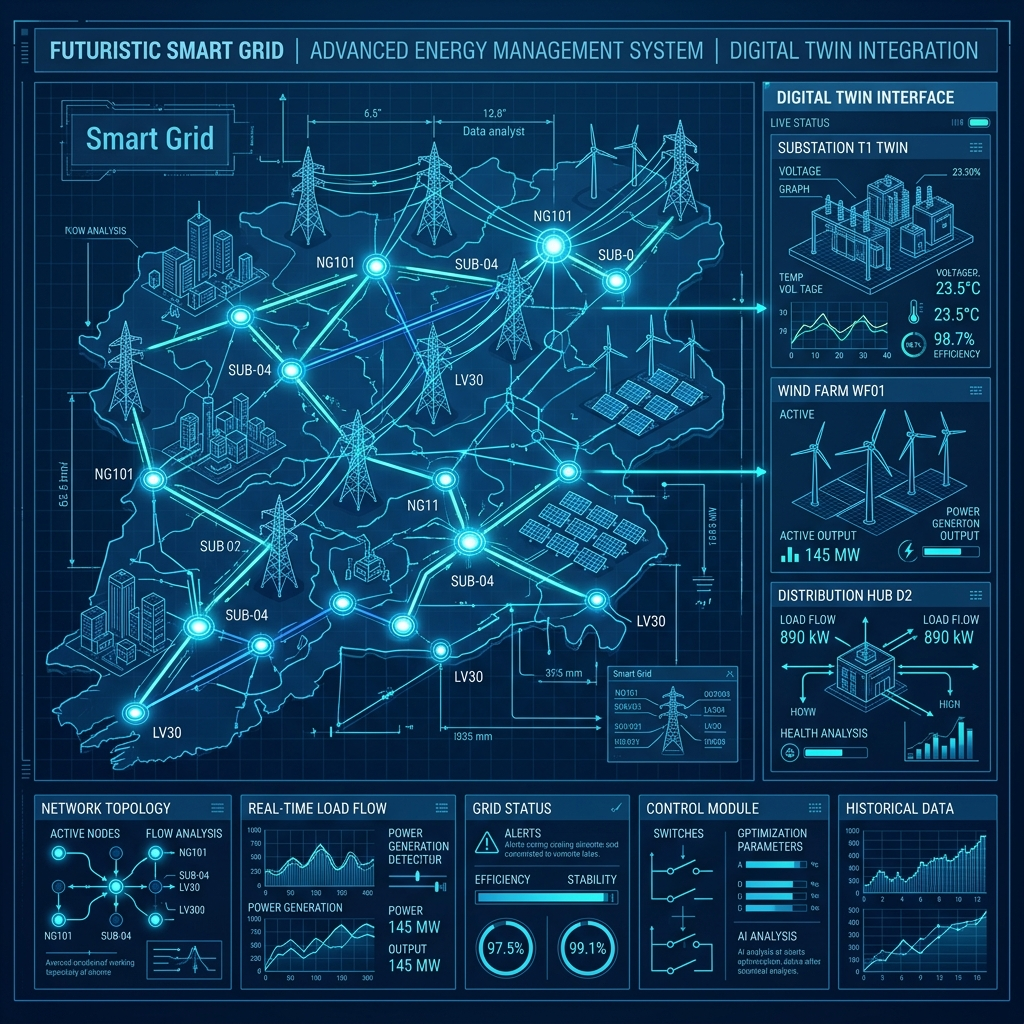
\includegraphics[width=0.6\textwidth]{figures/examples/smart_grid_ai.png}
  \caption{Mô hình trực quan hóa hệ thống lưới điện thông minh (Smart Grid)\protect\footnotemark}
  \label{fig:smart-grid-ai}
\end{figure}
\footnotetext{GHI CHÚ HỌC THUẬT QUAN TRỌNG: Hình ảnh minh họa này được tạo bởi AI (Generative AI). Theo quy định liêm chính học thuật, nếu sinh viên sử dụng hình ảnh do AI tạo sinh trong báo cáo/đồ án, BẮT BUỘC phải ghi rõ nguồn gốc trong chú thích hoặc footnote: \textit{"Hình ảnh được tạo bởi mô hình AI [Tên Model] với prompt chi tiết: [Nội dung prompt]"}. Ví dụ đối với hình này: Model: FLUX.1 / Prompt: \textit{"A futuristic high-tech Smart Grid power system with shining electrical nodes, transmission towers, and digital twins on a control dashboard interface, styled as a premium clean blueprint and technical schematic illustration..."}}

\subsection{Hình ảnh con (subfigure)}

\begin{lstlisting}[style=latexstyle, caption={Sử dụng subfigure}]
\begin{figure}[H]
  \centering
  \begin{subfigure}[b]{0.45\textwidth}
    \includegraphics[width=\textwidth]{hinh_a.png}
    \caption{Mo ta hinh a}
    \label{fig:sub-a}
  \end{subfigure}
  \hfill
  \begin{subfigure}[b]{0.45\textwidth}
    \includegraphics[width=\textwidth]{hinh_b.png}
    \caption{Mo ta hinh b}
    \label{fig:sub-b}
  \end{subfigure}
  \caption{Mo ta chung cho ca 2 hinh}
  \label{fig:both}
\end{figure}
\end{lstlisting}

Ví dụ chèn hệ hình con thực tế:
\begin{figure}[H]
  \centering
  \begin{subfigure}[b]{0.48\textwidth}
    \centering
    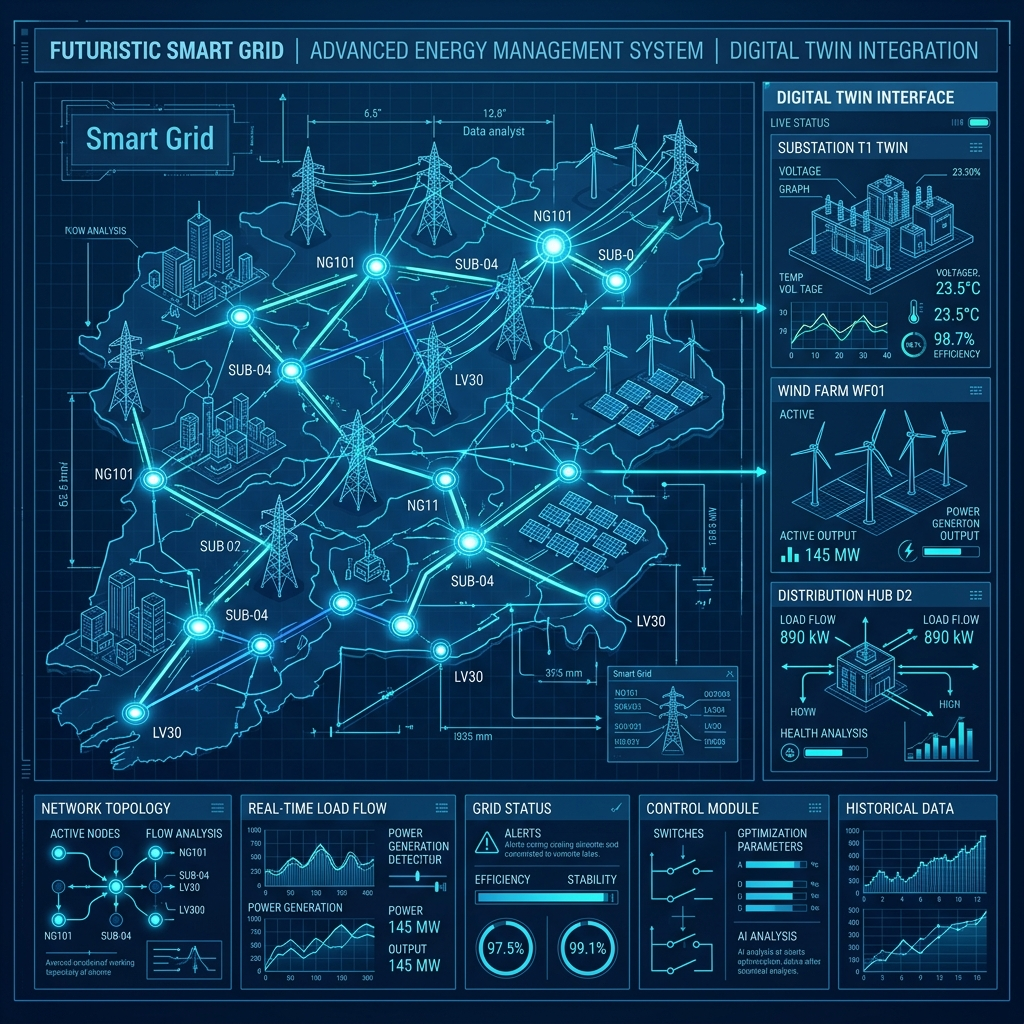
\includegraphics[width=\textwidth]{figures/examples/smart_grid_ai.png}
    \caption{Lưới điện thông minh}
    \label{fig:sub-smart-grid}
  \end{subfigure}
  \hfill
  \begin{subfigure}[b]{0.48\textwidth}
    \centering
    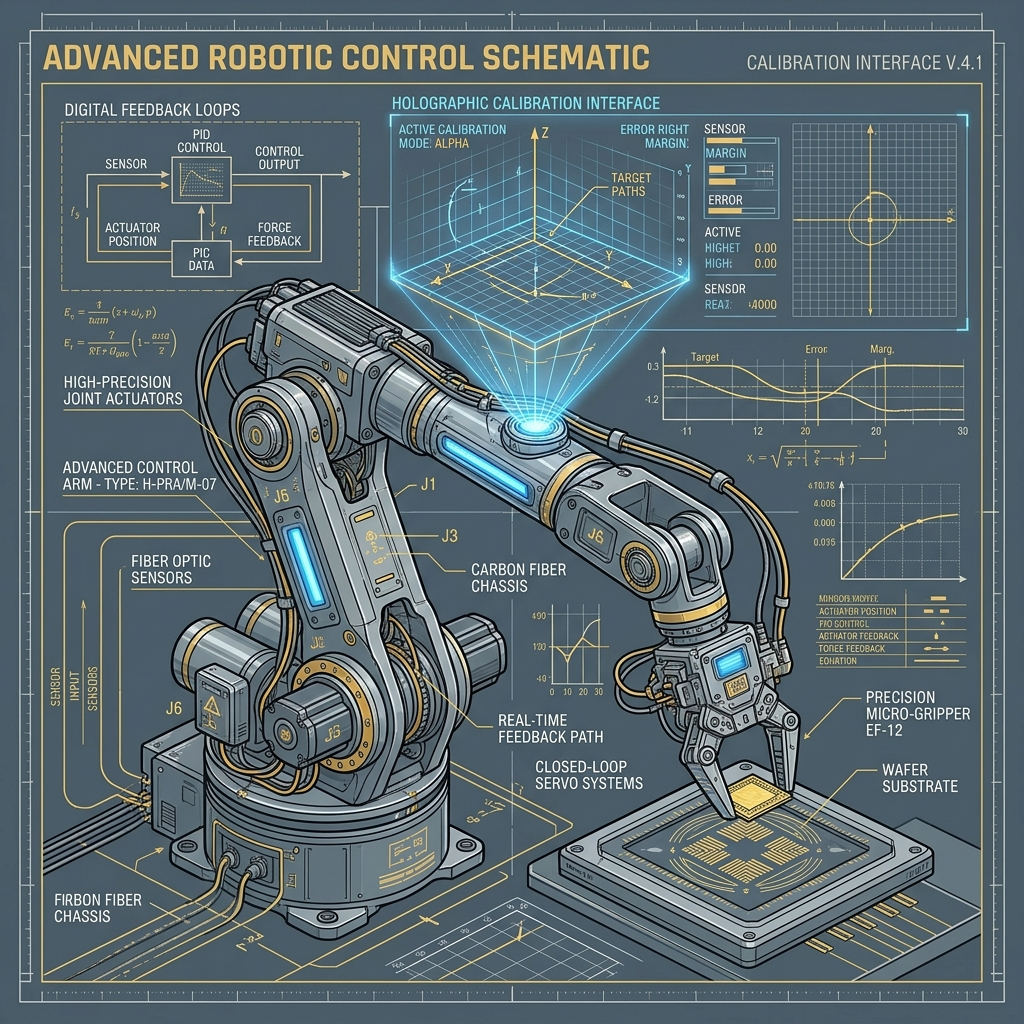
\includegraphics[width=\textwidth]{figures/examples/robotic_arm_ai.png}
    \caption{Cánh tay robot chính xác cao}
    \label{fig:sub-robotic-arm}
  \end{subfigure}
  \caption{Minh họa các thành phần hệ thống tự động hóa điện năng\protect\footnotemark}
  \label{fig:automation-components}
\end{figure}
\footnotetext{LƯU Ý LIÊM CHÍNH HỌC THUẬT VỀ HÌNH ẢNH AI: Tương tự như hình đơn, đối với hệ hình con (subfigure) có chứa ảnh do AI tạo sinh, sinh viên phải mô tả chi tiết nguồn gốc từng hình: (a) Lưới điện thông minh (Model: FLUX.1 / Prompt: \textit{"A futuristic high-tech Smart Grid..."}); (b) Cánh tay robot điều khiển (Model: FLUX.1 / Prompt: \textit{"A high-precision advanced robotic control arm..."}). Việc minh bạch nguồn gốc tài liệu là yếu tố sống còn trong nghiên cứu khoa học kỹ thuật.}

\subsection{Định dạng hình ảnh được hỗ trợ}

\begin{table}[H]
\centering
\caption{Các định dạng hình ảnh}
\label{tab:image-formats}
\begin{tabular}{llp{7cm}}
\toprule
\textbf{Định dạng} & \textbf{Khuyến nghị} & \textbf{Ghi chú} \\
\midrule
\texttt{.pdf} & $\bigstar\bigstar\bigstar$ & Vector, chất lượng cao nhất \\
\texttt{.eps} & $\bigstar\bigstar\bigstar$ & Vector, tự động chuyển sang PDF \\
\texttt{.png} & $\bigstar\bigstar$ & Bitmap, tốt cho ảnh chụp màn hình \\
\texttt{.jpg} & $\bigstar$ & Bitmap, tốt cho ảnh chụp, nén mất dữ liệu \\
\bottomrule
\end{tabular}
\end{table}

% ═══════════════════════════════════════════════════════════════
\section{Bảng biểu}
\label{sec:tables}

\subsection{Bảng đơn giản với booktabs}

\begin{lstlisting}[style=latexstyle, caption={Bảng với booktabs (khuyến nghị)}]
\begin{table}[H]
  \centering
  \caption{Ket qua thi nghiem}
  \label{tab:results}
  \begin{tabular}{lrr}
    \toprule
    \textbf{Phuong phap} & \textbf{Do chinh xac} & \textbf{Thoi gian} \\
    \midrule
    Phuong phap A & 95.2\% & 12.3s \\
    Phuong phap B & 97.8\% & 45.6s \\
    Phuong phap C & 96.5\% & 23.1s \\
    \bottomrule
  \end{tabular}
\end{table}
\end{lstlisting}

Ví dụ kết quả:

\begin{table}[H]
  \centering
  \caption{Kết quả thí nghiệm mẫu}
  \label{tab:sample-results}
  \begin{tabular}{lrr}
    \toprule
    \textbf{Phương pháp} & \textbf{Độ chính xác} & \textbf{Thời gian (s)} \\
    \midrule
    Phương pháp A & 95.2\% & 12.3 \\
    Phương pháp B & 97.8\% & 45.6 \\
    Phương pháp C & 96.5\% & 23.1 \\
    \bottomrule
  \end{tabular}
\end{table}

\subsection{Bảng dài (longtable)}

Dùng \texttt{longtable} cho bảng trải nhiều trang:

\begin{lstlisting}[style=latexstyle, caption={Bảng dài qua nhiều trang}]
\begin{longtable}{lll}
  \caption{Bang dai qua nhieu trang} \label{tab:long} \\
  \toprule
  \textbf{STT} & \textbf{Ten} & \textbf{Gia tri} \\
  \midrule
  \endfirsthead
  % Header lap lai o trang tiep theo
  \multicolumn{3}{c}{\textit{(Tiep theo trang truoc)}} \\
  \toprule
  \textbf{STT} & \textbf{Ten} & \textbf{Gia tri} \\
  \midrule
  \endhead
  1 & Muc 1 & 100 \\
  2 & Muc 2 & 200 \\
  % ... them cac dong khac
  \bottomrule
\end{longtable}
\end{lstlisting}

\subsection{Bảng ngang trang (landscape)}

\begin{lstlisting}[style=latexstyle, caption={Xoay bảng ngang trang}]
\begin{landscape}
\begin{table}
  \centering
  \caption{Bang rong can xoay ngang}
  \begin{tabular}{lllllllll}
    % ... noi dung bang rong ...
  \end{tabular}
\end{table}
\end{landscape}
\end{lstlisting}

% ═══════════════════════════════════════════════════════════════
\section{Công thức toán}
\label{sec:math}

\subsection{Công thức inline và display}

\begin{itemize}
  \item \textbf{Inline:} Dùng \verb|$...$| --- Ví dụ: $E = mc^2$
  \item \textbf{Display:} Dùng \verb|\[...\]| hoặc environment \texttt{equation}
\end{itemize}

\subsection{Công thức đánh số}

\begin{lstlisting}[style=latexstyle]
\begin{equation}
  P_{loss} = \sum_{k=1}^{N_{branch}} I_k^2 \cdot R_k
  \label{eq:ploss}
\end{equation}
\end{lstlisting}

Kết quả:
\begin{equation}
  P_{loss} = \sum_{k=1}^{N_{branch}} I_k^2 \cdot R_k
  \label{eq:ploss}
\end{equation}

Tham chiếu: ``Công thức~\eqref{eq:ploss} tính tổn thất công suất\ldots''

\subsection{Hệ phương trình (align)}

\begin{lstlisting}[style=latexstyle]
\begin{align}
  P_i &= V_i \sum_{j=1}^{N} V_j (G_{ij}\cos\theta_{ij}
         + B_{ij}\sin\theta_{ij}) \label{eq:pi} \\
  Q_i &= V_i \sum_{j=1}^{N} V_j (G_{ij}\sin\theta_{ij}
         - B_{ij}\cos\theta_{ij}) \label{eq:qi}
\end{align}
\end{lstlisting}

Kết quả:
\begin{align}
  P_i &= V_i \sum_{j=1}^{N} V_j (G_{ij}\cos\theta_{ij} + B_{ij}\sin\theta_{ij}) \label{eq:pi} \\
  Q_i &= V_i \sum_{j=1}^{N} V_j (G_{ij}\sin\theta_{ij} - B_{ij}\cos\theta_{ij}) \label{eq:qi}
\end{align}

\subsection{Ma trận}

\begin{lstlisting}[style=latexstyle]
\begin{equation}
  \mathbf{Y}_{bus} = \begin{bmatrix}
    Y_{11} & Y_{12} & \cdots & Y_{1n} \\
    Y_{21} & Y_{22} & \cdots & Y_{2n} \\
    \vdots & \vdots & \ddots & \vdots \\
    Y_{n1} & Y_{n2} & \cdots & Y_{nn}
  \end{bmatrix}
\end{equation}
\end{lstlisting}

Kết quả:
\begin{equation}
  \mathbf{Y}_{bus} = \begin{bmatrix}
    Y_{11} & Y_{12} & \cdots & Y_{1n} \\
    Y_{21} & Y_{22} & \cdots & Y_{2n} \\
    \vdots & \vdots & \ddots & \vdots \\
    Y_{n1} & Y_{n2} & \cdots & Y_{nn}
  \end{bmatrix}
  \label{eq:ybus}
\end{equation}

% ═══════════════════════════════════════════════════════════════
\section{Thuật toán (algorithm2e)}
\label{sec:algorithm}

\begin{lstlisting}[style=latexstyle, caption={Viết thuật toán}]
\begin{algorithm}[H]
  \caption{Ten thuat toan}
  \label{alg:sample}
  \KwIn{Du lieu dau vao}
  \KwOut{Ket qua dau ra}
  Khoi tao\;
  \For{$i = 1$ \KwTo $N$}{
    Tinh toan gia tri $f(x_i)$\;
    \If{$f(x_i) < f_{best}$}{
      $f_{best} \leftarrow f(x_i)$\;
    }
  }
  \Return $f_{best}$\;
\end{algorithm}
\end{lstlisting}

Ví dụ kết quả:

\begin{algorithm}[H]
  \caption{Thuật toán tối ưu hóa mẫu}
  \label{alg:sample}
  \KwIn{Quần thể ban đầu $X$, số vòng lặp $T_{max}$}
  \KwOut{Nghiệm tối ưu $x^*$}
  Khởi tạo quần thể ngẫu nhiên $X = \{x_1, x_2, \ldots, x_N\}$\;
  \For{$t = 1$ \KwTo $T_{max}$}{
    Tính giá trị hàm mục tiêu $f(x_i)$ cho mọi $i$\;
    \If{$f(x_i) < f_{best}$}{
      $x^* \leftarrow x_i$\;
      $f_{best} \leftarrow f(x_i)$\;
    }
    Cập nhật vị trí các cá thể\;
  }
  \Return $x^*$\;
\end{algorithm}

% ============================================================
%  HCMUT-DEE Thesis Kit v2.0.3 — Chương 4
%  Copyright (c) 2026 Nguyen Trong Thang & TS. Nguyen Phuc Khai
%  License: MIT
% ============================================================

\chapter{Quản Lý Tài Liệu Tham Khảo Chuẩn IEEE}
\label{ch:references}

\section{Tổng quan về BibTeX}

Template sử dụng \textbf{BibTeX} với style \texttt{IEEEtran} --- chuẩn trích dẫn được sử dụng rộng rãi nhất trong ngành Kỹ thuật Điện.

\begin{itemize}
  \item File \texttt{references.bib}: chứa tất cả tài liệu tham khảo.
  \item Mỗi entry có một \textbf{citation key} duy nhất (ví dụ: \texttt{nguyen2024optimal}).
  \item Trích dẫn trong văn bản bằng lệnh \verb|\cite{key}|.
\end{itemize}

\section{Cấu trúc file .bib}

\subsection{Bài báo tạp chí (@article)}

\begin{lstlisting}[style=latexstyle, caption={Entry @article mẫu}]
@article{nguyen2024optimal,
  title   = {Optimal Placement of DG in Distribution Networks},
  author  = {Nguyen, Van A and Tran, Van B},
  journal = {IEEE Transactions on Power Systems},
  volume  = {39},
  number  = {2},
  pages   = {1234--1245},
  year    = {2024},
  publisher = {IEEE}
}
\end{lstlisting}

\subsection{Bài conference (@inproceedings)}

\begin{lstlisting}[style=latexstyle, caption={Entry @inproceedings mẫu}]
@inproceedings{le2023method,
  title     = {A Novel Method for Power Flow Analysis},
  author    = {Le, Thi C and Pham, Van D},
  booktitle = {2023 IEEE PES General Meeting},
  pages     = {1--5},
  year      = {2023},
  publisher = {IEEE}
}
\end{lstlisting}

\subsection{Sách (@book)}

\begin{lstlisting}[style=latexstyle, caption={Entry @book mẫu}]
@book{glover2017power,
  title     = {Power Systems Analysis and Design},
  author    = {Glover, J. Duncan and Overbye, Thomas},
  year      = {2017},
  edition   = {6th},
  publisher = {Cengage Learning}
}
\end{lstlisting}

\subsection{Luận văn / Đồ án (@mastersthesis, @phdthesis)}

\begin{lstlisting}[style=latexstyle, caption={Entry luận văn mẫu}]
@mastersthesis{ntthang2025thesis,
  title  = {De xuat thua toan...},
  author = {Thang, Nguyen-Trong},
  school = {Truong Dai hoc Bach Khoa TP. HCM},
  year   = {2025}
}
\end{lstlisting}

\subsection{Website (@online hoặc @misc)}

\begin{lstlisting}[style=latexstyle, caption={Entry website mẫu}]
@misc{overleaf2024,
  title        = {Overleaf Documentation},
  author       = {{Overleaf}},
  howpublished = {\url{https://www.overleaf.com/learn}},
  year         = {2024},
  note         = {Truy cap: 2026-01-15}
}
\end{lstlisting}

\section{Cách trích dẫn trong văn bản}

\begin{table}[H]
\centering
\caption{Các lệnh trích dẫn}
\label{tab:cite-commands}
\begin{tabular}{lp{9cm}}
\toprule
\textbf{Lệnh} & \textbf{Kết quả / Ý nghĩa} \\
\midrule
\verb|\cite{key}|          & Trích dẫn 1 nguồn: [1] \\
\verb|\cite{key1,key2}|    & Trích dẫn nhiều nguồn: [1, 2] \\
\verb|\cite[p.~15]{key}|   & Trích dẫn có trang: [1, p. 15] \\
\bottomrule
\end{tabular}
\end{table}

\textbf{Quy ước đặt citation key:} \texttt{ho\_tac\_gia + nam + tu\_khoa}

Ví dụ: \texttt{nguyen2024optimal}, \texttt{glover2017power}, \texttt{ieee2019standard}

\subsection{Ví dụ thực tế trích dẫn sách giáo trình tiếng Việt}
Đối với sách giáo trình hoặc tài liệu tham khảo tiếng Việt có nhiều thông tin đặc thù (như thông tin tái bản, nhà xuất bản tiếng Việt), sinh viên cần nhập đầy đủ các trường thông tin tương tự như sách nước ngoài nhưng có thể Việt hóa các cụm từ cần thiết.

Ví dụ, sách giáo trình chuyên ngành Hệ thống điện của tác giả Hồ Văn Hiến~\cite{ho2005hethongdien} được khai báo trong file \texttt{references.bib} như sau:
\begin{lstlisting}[style=latexstyle, caption={Khai báo sách tiếng Việt mẫu trong .bib}]
@book{ho2005hethongdien,
  title={He thong dien: Truyen tai va phan phoi},
  author={Hien, Ho Van},
  year={2005},
  edition={tai ban lan thu nhat co sua chua, bo sung},
  publisher={Nha xuat ban Dai hoc Quoc gia TP. Ho Chi Minh},
  address={Thanh pho Ho Chi Minh}
}
\end{lstlisting}

Để trích dẫn sách này trong văn bản báo cáo, sinh viên chỉ cần gọi lệnh:
\begin{center}
  \texttt{\textbackslash cite\{ho2005hethongdien\}} $\rightarrow$ Kết quả hiển thị trong tài liệu: \cite{ho2005hethongdien}
\end{center}

\section{Lấy BibTeX nhanh}

\subsection{Từ Google Scholar}

\begin{enumerate}
  \item Tìm bài báo trên \url{https://scholar.google.com}
  \item Nhấn biểu tượng dấu ngoặc kép \textbf{``} (Cite)
  \item Chọn \textbf{BibTeX} ở cuối popup
  \item Copy và dán vào file \texttt{references.bib}
\end{enumerate}

\subsection{Từ Zotero / Mendeley}

\begin{enumerate}
  \item Import bài báo vào thư viện Zotero/Mendeley
  \item Export $\rightarrow$ chọn định dạng \textbf{BibTeX (.bib)}
  \item Copy nội dung vào file \texttt{references.bib}
\end{enumerate}

\section{Lưu ý thường gặp}

\begin{itemize}
  \item \textbf{Ký tự đặc biệt}: Dấu \texttt{\&} phải viết \verb|\&| trong BibTeX.
  \item \textbf{Chữ hoa trong title}: BibTeX có thể tự chuyển thành chữ thường. Để giữ chữ hoa, bọc trong \verb|{...}|. Ví dụ: \verb|title = {{IEEE} Standard}|.
  \item \textbf{Tên tiếng Việt}: Dùng dấu \verb|{...}| cho ký tự có dấu. Ví dụ: \verb|author = {Nguy{\~e}n, V{\u a}n A}|.
  \item \textbf{Kiểm tra}: Sau khi biên dịch, kiểm tra phần ``Tài liệu tham khảo'' xem có entry nào bị thiếu không (thường do typo trong citation key).
\end{itemize}

% ============================================================
%  HCMUT-DEE Thesis Kit v2.0.3 — Chương 5
%  Copyright (c) 2026 Nguyen Trong Thang & TS. Nguyen Phuc Khai
%  License: MIT
% ============================================================

\chapter{Phụ Lục, Mã Nguồn \& Listing Code}
\label{ch:code-listing}

\section{Viết phụ lục}

Phụ lục được khai báo sau lệnh \verb|\appendix| trong \texttt{thesis.tex}. Mỗi phụ lục là một \verb|\chapter{}| và được đánh ký hiệu A, B, C\ldots thay vì số.

\begin{lstlisting}[style=latexstyle, caption={Khai báo phụ lục}]
% Trong thesis.tex, sau phan Tai lieu tham khao:
\appendix
% ============================================================
%  HCMUT-DEE Thesis Kit v2.0.3 — Phụ lục mẫu
%  Copyright (c) 2026 Nguyen Trong Thang & TS. Nguyen Phuc Khai
%  License: MIT
% ============================================================

\chapter{Phụ lục mẫu}
\label{app:sample}

% ═══════════════════════════════════════════════════════════════
%  GHI CHU: Day la phu luc mau. Hay thay the bang noi dung
%  phu luc cua do an ban. Vi du: ma nguon, du lieu, bang phu.
% ═══════════════════════════════════════════════════════════════

\section{Ví dụ mã nguồn Python}

\begin{lstlisting}[style=pythonstyle, caption={Hàm tính tổn thất công suất trên lưới điện}, label={lst:app-python}]
import numpy as np

def backward_forward_sweep(R, X, P_load, Q_load, V_base=12.66):
    """
    Giai luu luong cong suat bang phuong phap
    Backward/Forward Sweep cho luoi hinh tia.
    """
    n_bus = len(P_load)
    V = np.ones(n_bus) * V_base  # Khoi tao dien ap

    for iteration in range(100):
        # Backward sweep: tinh dong nhanh
        I_branch = np.zeros(n_bus - 1, dtype=complex)
        for k in range(n_bus - 2, -1, -1):
            S = complex(P_load[k+1], Q_load[k+1])
            I_branch[k] = np.conj(S / V[k+1])

        # Forward sweep: cap nhat dien ap
        for k in range(n_bus - 1):
            Z = complex(R[k], X[k])
            V[k+1] = V[k] - I_branch[k] * Z

        # Kiem tra hoi tu
        if np.max(np.abs(V - V_old)) < 1e-6:
            break
        V_old = V.copy()

    return V
\end{lstlisting}

\section{Ví dụ bảng dữ liệu}

\begin{table}[H]
\centering
\caption{Thông số hệ thống IEEE 33-bus (trích một phần)}
\label{tab:app-ieee33}
\begin{tabular}{cccccc}
\toprule
\textbf{Nhánh} & \textbf{Từ} & \textbf{Đến} & \textbf{R ($\Omega$)} & \textbf{X ($\Omega$)} & \textbf{P$_{load}$ (kW)} \\
\midrule
1  & 1 & 2  & 0.0922 & 0.0477 & 100 \\
2  & 2 & 3  & 0.4930 & 0.2511 & 90  \\
3  & 3 & 4  & 0.3661 & 0.1864 & 120 \\
4  & 4 & 5  & 0.3811 & 0.1941 & 60  \\
5  & 5 & 6  & 0.8190 & 0.7070 & 60  \\
\bottomrule
\end{tabular}
\end{table}

% === CHEN FILE PDF BEN NGOAI (bo comment neu can) ===
% \section{Datasheet thiet bi}
% \includepdf[pages=-]{path/to/datasheet.pdf}
   % Phu luc A
% \input{appendices/appendix-b}       % Phu luc B (neu can)
\end{lstlisting}

\section{Chèn mã nguồn với listings}

Template đã định nghĩa sẵn \textbf{4 style} cho các ngôn ngữ phổ biến. Bạn chỉ cần chọn style phù hợp.

% ═══════════════════════════════════════════════════════════════
\subsection{Python (\texttt{pythonstyle})}

\begin{lstlisting}[style=pythonstyle, caption={Ví dụ mã Python --- Tính tổn thất công suất}, label={lst:python-sample}]
import numpy as np

def calculate_power_loss(V, I, R):
    """Tinh ton that cong suat tren luoi dien."""
    P_loss = np.sum(I**2 * R)
    print(f"Tong ton that: {P_loss:.2f} kW")
    return P_loss

# Tinh toan
voltage = np.array([1.0, 0.98, 0.95])
current = np.array([50.0, 45.0, 60.0])
resistance = np.array([0.01, 0.02, 0.015])
loss = calculate_power_loss(voltage, current, resistance)
\end{lstlisting}

% ═══════════════════════════════════════════════════════════════
\subsection{MATLAB (\texttt{matlabstyle})}

\begin{lstlisting}[style=matlabstyle, caption={Ví dụ mã MATLAB --- Giải hệ phương trình}, label={lst:matlab-sample}]
% Giai he phuong trinh tuyen tinh Ax = b
A = [4 -1 0; -1 4 -1; 0 -1 4];
b = [15; 10; 10];

% Phuong phap truc tiep
x = A \ b;

% Hien thi ket qua
fprintf('Nghiem x = [%.4f, %.4f, %.4f]\n', x);

% Ve do thi
figure;
plot(x, 'ro-', 'LineWidth', 2);
xlabel('Node'); ylabel('Voltage (p.u.)');
title('Voltage Profile');
grid on;
\end{lstlisting}

% ═══════════════════════════════════════════════════════════════
\subsection{C/C++ (\texttt{cstyle})}

\begin{lstlisting}[style=cstyle, caption={Ví dụ mã C --- Đọc ADC vi điều khiển}, label={lst:c-sample}]
#include <stdio.h>
#include <stdint.h>

#define ADC_RESOLUTION  4096    // 12-bit ADC
#define V_REF           3.3     // Dien ap tham chieu (V)

// Ham doc gia tri dien ap tu ADC
float read_voltage(uint16_t adc_value) {
    float voltage = (float)adc_value / ADC_RESOLUTION * V_REF;
    return voltage;
}

int main(void) {
    uint16_t raw = 2048;  // Gia tri ADC thu
    float v = read_voltage(raw);
    printf("Dien ap: %.3f V\n", v);
    return 0;
}
\end{lstlisting}

% ═══════════════════════════════════════════════════════════════
\subsection{PLC Structured Text (\texttt{plcstyle})}

\begin{lstlisting}[style=plcstyle, caption={Ví dụ PLC Structured Text --- Điều khiển động cơ}, label={lst:plc-sample}]
PROGRAM Motor_Control
VAR
    Start_Button  : BOOL := FALSE;
    Stop_Button   : BOOL := FALSE;
    Motor_Running : BOOL := FALSE;
    Speed_SP      : REAL := 1500.0;    (* Toc do dat (RPM) *)
    Speed_PV      : REAL := 0.0;       (* Toc do thuc te *)
    Timer_Delay   : TON;               (* Bo dinh thoi *)
END_VAR

(* Logic dieu khien chinh *)
IF Start_Button AND NOT Stop_Button THEN
    Timer_Delay(IN := TRUE, PT := T#2S);
    IF Timer_Delay.Q THEN
        Motor_Running := TRUE;
    END_IF;
ELSIF Stop_Button THEN
    Motor_Running := FALSE;
    Timer_Delay(IN := FALSE);
END_IF;

END_PROGRAM
\end{lstlisting}

% ═══════════════════════════════════════════════════════════════
\section{Chèn file code bên ngoài}

Thay vì copy code vào file \texttt{.tex}, bạn có thể include trực tiếp:

\begin{lstlisting}[style=latexstyle, caption={Chèn file code bên ngoài}]
% Chen file Python
\lstinputlisting[style=pythonstyle,
  caption={Ma nguon chuong trinh chinh},
  label={lst:main-py}
]{path/to/main.py}

% Chen 1 phan cua file (dong 10 den 25)
\lstinputlisting[style=matlabstyle,
  firstline=10, lastline=25,
  caption={Ham tinh luu luong cong suat}
]{path/to/powerflow.m}
\end{lstlisting}

% ═══════════════════════════════════════════════════════════════
\section{Đính kèm PDF bên ngoài}

Dùng package \texttt{pdfpages} để chèn file PDF (datasheet, chứng chỉ, \ldots):

\begin{lstlisting}[style=latexstyle, caption={Chèn file PDF bên ngoài}]
% Chen tat ca cac trang cua file PDF
\includepdf[pages=-]{path/to/document.pdf}

% Chi chen trang 1 va 3
\includepdf[pages={1,3}]{path/to/document.pdf}

% Chen voi tieu de
\includepdf[pages=-, pagecommand={
  \thispagestyle{fancy}}]{path/to/datasheet.pdf}
\end{lstlisting}

% ============================================================
%  HCMUT-DEE Thesis Kit v2.0.3 — Chương 6
%  Copyright (c) 2026 Nguyen Trong Thang & TS. Nguyen Phuc Khai
%  License: MIT
% ============================================================

\chapter{FAQ, Mẹo \& Xử Lý Lỗi Thường Gặp}
\label{ch:faq}

\section{Lỗi biên dịch phổ biến}

\subsection{Undefined control sequence}

\textbf{Nguyên nhân:} Gõ sai tên lệnh hoặc thiếu package.

\begin{lstlisting}[style=latexstyle, caption={Ví dụ lỗi và cách sửa}]
% SAI (thieu dau \)
\begin{itemze}   % -> Undefined control sequence

% DUNG
\begin{itemize}
\end{lstlisting}

\textbf{Cách sửa:} Kiểm tra chính tả tên lệnh. Nếu đúng chính tả, kiểm tra xem package tương ứng đã được load chưa.

\subsection{Missing \$ inserted}

\textbf{Nguyên nhân:} Sử dụng ký tự toán học bên ngoài chế độ toán.

\begin{lstlisting}[style=latexstyle]
% SAI
Dien ap V_i tai nut i         % -> Missing $

% DUNG
Dien ap $V_i$ tai nut $i$
\end{lstlisting}

\subsection{File not found}

\textbf{Nguyên nhân:} Đường dẫn hình ảnh hoặc file sai.

\begin{lstlisting}[style=latexstyle]
% SAI (duong dan sai)
\includegraphics{Figures/hinh1.png}  % F hoa

% DUNG (dung nhu trong folder)
\includegraphics{figures/hinh1.png}  % f thuong
\end{lstlisting}

\textbf{Lưu ý:} Linux/Overleaf phân biệt chữ hoa/thường, Windows thì không.

\subsection{LaTeX Error: Too many unprocessed floats}

\textbf{Nguyên nhân:} Quá nhiều hình/bảng liên tiếp mà không có đoạn văn bản.

\textbf{Cách sửa:} Thêm \verb|\clearpage| giữa các hình/bảng, hoặc dùng \verb|[H]| từ package \texttt{float}.

% ═══════════════════════════════════════════════════════════════
\section{Bảng tràn lề}

\textbf{Giải pháp theo mức độ:}

\begin{enumerate}
  \item \textbf{Thu nhỏ font:} Thêm \verb|\small| hoặc \verb|\footnotesize| trước bảng.
  \item \textbf{Dùng tabularx:} Cột \texttt{X} tự co giãn.
  \item \textbf{Xoay ngang:} Dùng \verb|\begin{landscape}...\end{landscape}|.
  \item \textbf{Chia bảng:} Tách thành 2 bảng nhỏ hơn.
\end{enumerate}

\begin{lstlisting}[style=latexstyle, caption={Dùng tabularx để bảng tự co giãn}]
\begin{table}[H]
\centering\small
\begin{tabularx}{\textwidth}{lXXr}
  \toprule
  \textbf{STT} & \textbf{Mo ta dai} & \textbf{Chi tiet} & \textbf{Gia tri} \\
  \midrule
  1 & Noi dung tu dong xuong dong & Chi tiet bo sung & 100 \\
  \bottomrule
\end{tabularx}
\end{table}
\end{lstlisting}

% ═══════════════════════════════════════════════════════════════
\section{Font tiếng Việt bị lỗi}

\textbf{Triệu chứng:} Chữ có dấu hiển thị sai hoặc mất dấu.

\textbf{Kiểm tra:}
\begin{enumerate}
  \item File \texttt{.tex} đã lưu encoding \textbf{UTF-8} chưa?
  \item Đã dùng option \texttt{[vietnamese]} trong \verb|\documentclass|?
  \item Trên Overleaf: kiểm tra ``Menu $\rightarrow$ Compiler: pdfLaTeX''.
\end{enumerate}

% ═══════════════════════════════════════════════════════════════
\section{Overleaf timeout}

Overleaf giới hạn thời gian biên dịch (miễn phí: 1 phút). Nếu bị timeout:

\begin{itemize}
  \item Giảm số hình ảnh có dung lượng lớn (nén PNG $\rightarrow$ JPG).
  \item Dùng \verb|\input{}| thay vì \verb|\include{}| (nhanh hơn).
  \item Comment tạm các chương chưa viết xong.
  \item Chuyển hình \texttt{.eps} sang \texttt{.pdf} trước khi upload.
  \item Xóa file \texttt{.aux}, \texttt{.log} cũ.
\end{itemize}

% ═══════════════════════════════════════════════════════════════
\section{Mẹo hay}

\subsection{\texttt{\textbackslash input} vs \texttt{\textbackslash include}}

\begin{table}[H]
\centering
\caption{So sánh \texttt{\textbackslash input} và \texttt{\textbackslash include}}
\label{tab:input-vs-include}
\begin{tabular}{lp{5.5cm}p{5.5cm}}
\toprule
 & \texttt{\textbackslash input\{file\}} & \texttt{\textbackslash include\{file\}} \\
\midrule
\textbf{Chức năng} & Chèn trực tiếp nội dung & Chèn + tự thêm \verb|\clearpage| \\
\textbf{Tốc độ} & Nhanh hơn & Chậm hơn (tạo file .aux riêng) \\
\textbf{Dùng cho} & Section, phần nhỏ & Chương riêng biệt \\
\textbf{Lồng nhau} & Được & Không được \\
\bottomrule
\end{tabular}
\end{table}

\textbf{Khuyến nghị:} Dùng \verb|\input{}| cho hầu hết trường hợp.

\subsection{Backup với Git}

\begin{lstlisting}[style=latexstyle, caption={Các lệnh Git cơ bản}]
git init                          % Khoi tao repo
git add .                         % Them tat ca file
git commit -m "Xong chuong 3"    % Luu phien ban
git push origin main              % Day len GitHub/GitLab
\end{lstlisting}

\subsection{Compile nhanh hơn}

Khi đang viết, chỉ cần chạy \texttt{pdflatex} \textbf{1 lần} (không cần bibtex). Chạy đầy đủ 4 bước khi cần cập nhật tài liệu tham khảo.

% ═══════════════════════════════════════════════════════════════
\section{Sử dụng AI hỗ trợ viết đồ án}

Bạn có thể dùng ChatGPT, Gemini, hoặc Claude để hỗ trợ viết nội dung. Xem file \texttt{prompts/ai-writing-prompt.md} để có prompt mẫu chi tiết.

\textbf{Ví dụ prompt:}

\begin{tcolorbox}[title={Prompt mẫu cho AI}, colback=CodeBG]
\small
``Tôi đang viết đồ án tốt nghiệp bằng LaTeX, dùng template HCMUT-DEE Thesis Kit. Hãy giúp tôi viết phần Cơ sở lý thuyết (Chương 2) về lưới điện phân phối hình tia. Viết bằng tiếng Việt, văn phong học thuật, có trích dẫn giả [X]. Output phải là mã LaTeX sẵn sàng paste vào file chapter2.tex.''
\end{tcolorbox}

% ═══════════════════════════════════════════════════════════════
\section{Liên hệ \& đóng góp}

Nếu bạn gặp lỗi hoặc muốn đóng góp cải tiến template:

\begin{itemize}
  \item Tạo \textbf{Issue} hoặc \textbf{Pull Request} trên GitHub repository.
  \item Liên hệ tác giả: Nguyễn Trọng Thắng (K19 --- Hệ thống điện).
\end{itemize}

\begin{center}
  \textit{Chúc bạn hoàn thành đồ án tốt nghiệp xuất sắc!}
\end{center}


% ─── TAI LIEU THAM KHAO ─────────────────────────────────────
\bibliographystyle{IEEEtran}
\bibliography{references}

% ─── PHU LUC ─────────────────────────────────────────────────
\appendix
% ============================================================
%  HCMUT-DEE Thesis Kit v2.0.3 — Phụ lục mẫu
%  Copyright (c) 2026 Nguyen Trong Thang & TS. Nguyen Phuc Khai
%  License: MIT
% ============================================================

\chapter{Phụ lục mẫu}
\label{app:sample}

% ═══════════════════════════════════════════════════════════════
%  GHI CHU: Day la phu luc mau. Hay thay the bang noi dung
%  phu luc cua do an ban. Vi du: ma nguon, du lieu, bang phu.
% ═══════════════════════════════════════════════════════════════

\section{Ví dụ mã nguồn Python}

\begin{lstlisting}[style=pythonstyle, caption={Hàm tính tổn thất công suất trên lưới điện}, label={lst:app-python}]
import numpy as np

def backward_forward_sweep(R, X, P_load, Q_load, V_base=12.66):
    """
    Giai luu luong cong suat bang phuong phap
    Backward/Forward Sweep cho luoi hinh tia.
    """
    n_bus = len(P_load)
    V = np.ones(n_bus) * V_base  # Khoi tao dien ap

    for iteration in range(100):
        # Backward sweep: tinh dong nhanh
        I_branch = np.zeros(n_bus - 1, dtype=complex)
        for k in range(n_bus - 2, -1, -1):
            S = complex(P_load[k+1], Q_load[k+1])
            I_branch[k] = np.conj(S / V[k+1])

        # Forward sweep: cap nhat dien ap
        for k in range(n_bus - 1):
            Z = complex(R[k], X[k])
            V[k+1] = V[k] - I_branch[k] * Z

        # Kiem tra hoi tu
        if np.max(np.abs(V - V_old)) < 1e-6:
            break
        V_old = V.copy()

    return V
\end{lstlisting}

\section{Ví dụ bảng dữ liệu}

\begin{table}[H]
\centering
\caption{Thông số hệ thống IEEE 33-bus (trích một phần)}
\label{tab:app-ieee33}
\begin{tabular}{cccccc}
\toprule
\textbf{Nhánh} & \textbf{Từ} & \textbf{Đến} & \textbf{R ($\Omega$)} & \textbf{X ($\Omega$)} & \textbf{P$_{load}$ (kW)} \\
\midrule
1  & 1 & 2  & 0.0922 & 0.0477 & 100 \\
2  & 2 & 3  & 0.4930 & 0.2511 & 90  \\
3  & 3 & 4  & 0.3661 & 0.1864 & 120 \\
4  & 4 & 5  & 0.3811 & 0.1941 & 60  \\
5  & 5 & 6  & 0.8190 & 0.7070 & 60  \\
\bottomrule
\end{tabular}
\end{table}

% === CHEN FILE PDF BEN NGOAI (bo comment neu can) ===
% \section{Datasheet thiet bi}
% \includepdf[pages=-]{path/to/datasheet.pdf}

% ============================================================
%  HCMUT-DEE Thesis Kit v2.0.4 — Phụ lục B
%  Copyright (c) 2026 Nguyễn Trọng Thắng & TS. Nguyễn Phúc Khải
%  License: MIT
% ============================================================

\chapter{Danh sách lệnh và Hướng dẫn sử dụng nhanh}
\label{app:commands-guide}

Phụ lục này tổng hợp toàn bộ danh sách các lệnh tùy biến (custom commands), biến dữ liệu học viên (metadata) và các kiểu định dạng có sẵn trong lớp tài liệu \texttt{hcmut-dee.cls}. Sinh viên có thể tra cứu nhanh để tùy biến báo cáo của mình.

\section{Các lệnh khai báo thông tin học viên (Metadata)}

Mở file \texttt{thesis.tex} để chỉnh sửa các thông tin này trong phần ``THÔNG TIN SINH VIÊN''.

\subsection{Khai báo bắt buộc}
\begin{itemize}
  \item \verb|\ThesisTitle{...}|: Khai báo tiêu đề đồ án tốt nghiệp bằng tiếng Việt.
  \item \verb|\ThesisTitleEN{...}|: Khai báo tiêu đề tiếng Anh tương ứng.
  \item \verb|\StudentName{...}|: Khai báo Họ và tên sinh viên thực hiện.
  \item \verb|\StudentID{...}|: Khai báo Mã số sinh viên (MSSV).
  \item \verb|\StudentClass{...}|: Khai báo Lớp sinh hoạt (ví dụ: \texttt{BK21HTD}).
  \item \verb|\Major{...}|: Khai báo Ngành đào tạo (ví dụ: \texttt{Kỹ thuật Điện}).
  \item \verb|\Supervisor{...}|: Khai báo Học hàm, học vị và họ tên Giảng viên hướng dẫn.
\end{itemize}

\subsection{Khai báo tùy chọn (Có sẵn giá trị mặc định)}
\begin{itemize}
  \item \verb|\Faculty{...}|: Khai báo tên Khoa quản lý (Mặc định: \texttt{Khoa Điện - Điện Tử}).
  \item \verb|\Department{...}|: Khai báo tên Bộ môn (Ví dụ: \texttt{Bộ môn Hệ thống điện}).
  \item \verb|\ReportType{...}|: Khai báo loại báo cáo (Mặc định: \texttt{ĐỒ ÁN TỐT NGHIỆP}).
  \item \verb|\ThesisMonth{...}|: Khai báo tháng bảo vệ (Định dạng hai chữ số, ví dụ: \texttt{06}).
  \item \verb|\ThesisYear{...}|: Khai báo năm bảo vệ (Định dạng bốn chữ số, ví dụ: \texttt{2026}).
  \item \verb|\AssignDate{ngay}{thang}{nam}|: Khai báo ngày giao nhiệm vụ đồ án tốt nghiệp.
  \item \verb|\DueDate{ngay}{thang}{nam}|: Khai báo ngày hạn cuối nộp báo cáo.
  \item \verb|\Reviewer{...}|: Khai báo Giảng viên phản biện (nếu biết trước).
  \item \verb|\SupervisorPercent{...}|: Tỷ lệ hướng dẫn của GVHD (Mặc định: \texttt{100\%}).
  \item \verb|\AssignmentTasks{...}|: Khai báo danh sách các đầu việc chính trong trang Nhiệm vụ.
\end{itemize}

\subsection{Khai báo thành viên Hội đồng chấm (Mới bổ sung)}
Để hiển thị tên Hội đồng trên trang Tờ chấm điểm, hãy bỏ dấu comment \texttt{\%} ở các dòng sau trong \texttt{thesis.tex}:
\begin{itemize}
  \item \verb|\CouncilMemberOne{...}|: Khai báo họ tên Chủ tịch Hội đồng.
  \item \verb|\CouncilMemberTwo{...}|: Khai báo họ tên Ủy viên/Thư ký Hội đồng.
  \item \verb|\CouncilMemberThree{...}|: Khai báo họ tên Ủy viên thứ 3.
  \item \verb|\CouncilMemberFour{...}|: Khai báo họ tên Ủy viên thứ 4.
  \item \verb|\CouncilMemberFive{...}|: Khai báo họ tên Ủy viên thứ 5.
\end{itemize}

\section{Các lệnh sinh trang tự động (Page Generators)}

Các lệnh này được gọi trong \texttt{thesis.tex} để tự động tạo ra các trang giấy tờ biểu mẫu hành chính chuẩn quy định:
\begin{itemize}
  \item \verb|\makecover|: Sinh trang bìa chính thức có hoa văn viền khung kép Bách Khoa.
  \item \verb|\makeassignment|: Sinh trang Nhiệm vụ khóa luận/đồ án tốt nghiệp theo form FL012.
  \item \verb|\makeevaluation|: Sinh trang tờ chấm điểm hội đồng (Tự động hiển thị tên hoặc kẻ hàng chấm chấm điền tay).
\end{itemize}

\section{Các lệnh lấy dữ liệu an toàn (Public Getters)}

Sinh viên có thể sử dụng các lệnh sau trong văn bản để hiển thị các dữ liệu đã khai báo ở phần thông tin sinh viên mà không bị dính ký tự đặc biệt \texttt{@}:
\begin{center}
\begin{tabular}{ll}
  \toprule
  \textbf{Lệnh truy xuất} & \textbf{Thông tin lấy ra} \\
  \midrule
  \verb|\getThesisTitle|    & Tiêu đề đề tài bằng tiếng Việt \\
  \verb|\getThesisTitleEN|  & Tiêu đề đề tài bằng tiếng Anh \\
  \verb|\getStudentName|     & Họ tên sinh viên thực hiện \\
  \verb|\getStudentID|       & Mã số sinh viên (MSSV) \\
  \verb|\getStudentClass|    & Lớp sinh hoạt \\
  \verb|\getMajor|           & Ngành đào tạo \\
  \verb|\getSupervisor|      & Giảng viên hướng dẫn \\
  \verb|\getFaculty|         & Tên Khoa chủ quản \\
  \verb|\getThesisMonth|     & Tháng bảo vệ đề tài \\
  \verb|\getThesisYear|      & Năm bảo vệ đề tài \\
  \verb|\getCouncilMemberOne| & Họ tên Chủ tịch Hội đồng chấm \\
  \verb|\getCouncilMemberTwo| & Họ tên Ủy viên/Thư ký Hội đồng \\
  \verb|\getCouncilMemberThree| & Họ tên Ủy viên thứ 3 \\
  \verb|\getCouncilMemberFour| & Họ tên Ủy viên thứ 4 \\
  \verb|\getCouncilMemberFive| & Họ tên Ủy viên thứ 5 \\
  \bottomrule
\end{tabular}
\end{center}

\section{Các kiểu định dạng mã nguồn (Code Listings Styles)}

Template được cấu hình sẵn 5 môi trường định dạng mã nguồn trong khối lệnh \verb|\begin{lstlisting}[style=...]|:
\begin{enumerate}
  \item \texttt{pythonstyle}: Tối ưu hóa từ khóa chuyên sâu cho mã nguồn Python.
  \item \texttt{matlabstyle}: Tối ưu hóa từ khóa và ký hiệu cho mã nguồn MATLAB.
  \item \texttt{cstyle}: Tối ưu hóa định dạng cho ngôn ngữ C/C++ và các định dạng kiểu dữ liệu nhúng.
  \item \texttt{plcstyle}: Định dạng từ khóa Structured Text (IEC 61131-3) chuyên biệt cho ngành Điện - Điện tử.
  \item \texttt{latexstyle}: Hỗ trợ viết và giải thích các thẻ lệnh LaTeX.
\end{enumerate}

\section{Quy trình biên dịch 4 bước tiêu chuẩn}

Để đảm bảo mục lục, tham chiếu và danh mục tài liệu tham khảo được cập nhật chính xác nhất, quy trình biên dịch thủ công qua terminal gồm các lệnh sau:
\begin{lstlisting}[style=latexstyle, caption={Quy trinh bien dich 4 buoc qua Terminal}]
pdflatex thesis.tex
bibtex thesis
pdflatex thesis.tex
pdflatex thesis.tex
\end{lstlisting}
\textit{Lưu ý: Nếu sử dụng Overleaf, hệ thống sẽ tự động thực hiện đầy đủ các bước này khi nhấn nút Recompile.}

\chapter{Công cụ CLI quản lý luận văn (Thesis Tool)}
\label{appendix:cli-tool}

Nhằm mang lại sự tiện lợi, tự động hóa và dễ dàng sử dụng cho người dùng trong quá trình làm luận văn, một công cụ dòng lệnh (CLI - Command Line Interface) nhỏ gọn đã được phát triển chuyên biệt cho bộ mẫu template này. Công cụ này được viết bằng ngôn ngữ Golang để tận dụng khả năng biên dịch thành một tập tin thực thi duy nhất (.exe) mà không cần phải cài đặt môi trường Go, đảm bảo tính nhẹ gọn và khả năng thực thi nhanh chóng.

\section{Mục đích và Ưu điểm}
\begin{itemize}
    \item \textbf{Tự động hóa quá trình biên dịch:} Thay vì phải chạy tuần tự các lệnh \texttt{pdflatex}, \texttt{biber}, và \texttt{pdflatex} nhiều lần theo cách thủ công, công cụ tự động lo liệu quy trình này với cấu hình chuẩn nhất.
    \item \textbf{Dọn dẹp tự động:} Cung cấp tính năng xóa các tập tin tạm, file rác (\texttt{.aux, .log, .toc, .bbl}, v.v.) sinh ra sau quá trình biên dịch, giúp thư mục mã nguồn luôn sạch sẽ.
    \item \textbf{Đóng gói trực tiếp, độc lập:} Công cụ đã được biên dịch sẵn thành tập tin \texttt{thesis-tool.exe} duy nhất. Sinh viên chỉ việc chạy và sử dụng mà không cần hiểu biết về Golang.
\end{itemize}

\section{Danh sách các lệnh hỗ trợ}
Để sử dụng công cụ, mở Terminal hoặc Command Prompt tại thư mục gốc của dự án (nơi chứa file \texttt{thesis-tool.exe}) và sử dụng các lệnh sau:

\begin{enumerate}
    \item \textbf{Biên dịch luận văn (Build)}
    \begin{verbatim}
    thesis-tool build
    \end{verbatim}
    Lệnh này sẽ tiến hành gọi trình biên dịch LaTeX để dịch file \texttt{thesis/thesis.tex} sang PDF. Quá trình bao gồm các bước biên dịch văn bản, trích xuất tài liệu tham khảo với Biber và cập nhật lại mục lục. File kết quả sẽ là \texttt{thesis/thesis.pdf}.

    \item \textbf{Dọn dẹp thư mục (Clean)}
    \begin{verbatim}
    thesis-tool clean
    \end{verbatim}
    Sử dụng lệnh này khi muốn xóa các tập tin tạm, file log và các tệp hỗ trợ phụ được sinh ra trong quá trình biên dịch nhằm giải phóng dung lượng và giúp dự án gọn gàng.

    \item \textbf{Xem phiên bản (Version)}
    \begin{verbatim}
    thesis-tool version
    \end{verbatim}
    Hiển thị thông tin phiên bản hiện tại của bộ công cụ, ở bản cập nhật này là \textbf{v2.0.4}.

    \item \textbf{Xem trợ giúp (Help)}
    \begin{verbatim}
    thesis-tool help
    \end{verbatim}
    Liệt kê và giải thích ngắn gọn cách dùng của tất cả các lệnh được hỗ trợ.
\end{enumerate}

Với \texttt{thesis-tool}, việc tương tác và phát triển luận văn trên template sẽ trở nên hiện đại, chuyên nghiệp và tiết kiệm thời gian hơn rất nhiều.


\end{document}
